\documentclass{article}
\usepackage[preprint]{vendor/neurips_2026}
\usepackage{fontspec}
\setmainfont{texgyretermes-regular.otf}[
  BoldFont=texgyretermes-bold.otf,
  ItalicFont=texgyretermes-italic.otf,
  BoldItalicFont=texgyretermes-bolditalic.otf]
\setsansfont{texgyreheros-regular.otf}[
  BoldFont=texgyreheros-bold.otf,
  ItalicFont=texgyreheros-italic.otf,
  BoldItalicFont=texgyreheros-bolditalic.otf]
\setmonofont{JuliaMono-Regular.ttf}[
  Ligatures=NoCommon,Scale=0.9,
  BoldFont=JuliaMono-Bold.ttf,
  ItalicFont=JuliaMono-RegularItalic.ttf,
  BoldItalicFont=JuliaMono-BoldItalic.ttf]
\usepackage{amsmath,amssymb,amsthm,mathtools}
\usepackage{booktabs,fvextra,microtype,xcolor,longtable,graphicx}
\usepackage[unicode,hidelinks]{hyperref}
\usepackage{enumitem,placeins,pgfplots}
\pgfplotsset{compat=1.18}
\AddToHook{shipout/background}{%
  \begin{tikzpicture}[remember picture,overlay]
    \node[rotate=45,text=black!12,
      font=\sffamily\bfseries\fontsize{64}{64}\selectfont]
      at (current page.center) {AI-generated};
  \end{tikzpicture}%
}
\setlist{nosep,leftmargin=*}
\fvset{fontsize=\small,breaklines=true,breaksymbolleft={},breaksymbolright={}}
\newtheorem{theorem}{Theorem}
\newtheorem{lemma}{Lemma}
\newtheorem{proposition}{Proposition}
\newcommand{\R}{\mathbb{R}}
\newcommand{\Q}{\mathbb{Q}}
\newcommand{\norm}[1]{\left\lVert#1\right\rVert}
\newcommand{\NA}{\texttt{norm\_arith}}
\newcommand{\sourcepath}[1]{\texttt{\detokenize{#1}}}
\newcommand{\CensusFiles}{8637}
\newcommand{\CensusComplete}{8610}
\newcommand{\CensusFailed}{27}
\newcommand{\CensusEligible}{20628}
\newcommand{\CensusProposals}{40}
\newcommand{\CensusUnknown}{99}
\newcommand{\PatchReplacements}{87}
\newcommand{\PatchFiles}{46}
\newcommand{\PatchBefore}{582}
\newcommand{\PatchAfter}{226}
\newcommand{\PatchProofSaved}{356}
\newcommand{\PatchNetSaved}{310}
\newcommand{\PatchImports}{46}
\newcommand{\CaseID}{manual-strong-law-sums}
\newcommand{\CaseBefore}{20}
\newcommand{\CaseAfter}{5}
\newcommand{\FollowupFiles}{885}
\newcommand{\FollowupComplete}{875}
\newcommand{\FollowupFailed}{10}
\newcommand{\FollowupProposals}{158}
\newcommand{\StudyRatio}{1.0724}
\newcommand{\StudyLower}{1.0669}
\newcommand{\StudyUpper}{1.0814}
\newcommand{\StudyOriginal}{131.188}
\newcommand{\StudyReplacement}{122.333}

\title{From a Community Request to a Lean Tactic:\\AI-Assisted Norm Arithmetic}
\author{Anonymous Authors}
\date{}

\begin{document}
\maketitle
\begin{abstract}
A 2020 Lean community discussion asked for automation that finds hidden decompositions in norm inequalities.
We used artificial intelligence (AI) coding agents to develop \NA{}, a reusable Lean tactic for the normed-space part of this request.
AI assisted development.
The resulting tactic runs without a language model and constructs proofs that Lean checks.
We give the implementation, its finite real-space core, and an evaluation against existing mathlib proofs.

The core handles rational vector terms and affine scalar comparisons with norms.
Bounded extensions handle local quantified bounds and finite metric constraints.

A verified local patch replaces \PatchReplacements{} proof spans in \PatchFiles{} files and removes \PatchNetSaved{} code lines after preparation and imports.
Across 40 paired passes with built dependencies, the ratio of mean original and replacement compilation times is \StudyRatio{}.
The conditional paired 95\% interval is $[\StudyLower{},\StudyUpper{}]$.
This case study measures the resulting artifact, without a controlled comparison of AI and human development effort.
\end{abstract}

\section{A community request for norm automation}
\label{sec:problem}
In May 2020, Heather Macbeth asked for a Lean tactic that could find decompositions for norm inequalities \citep{leanrequest2020}.
The example was $\norm{2a+b}\le3\norm{a}+\norm{b-a}$.
Its useful identity is $2a+b=3a+(b-a)$.
The discussion identified this decomposition search as a missing step in automation.
The later discussion also proposed normed-algebra reasoning with products, which remains outside our core.
We address the decomposition-search part of the request.

We used AI coding agents to build a reusable tactic for this kind of proof.
The resulting \NA{} finds rational coefficients and constructs a proof from them.
This checked source example proves the requested inequality.
Here $E$ is a real seminormed space.
\VerbatimInput{generated/community-request.lean}


The supplied facts give bounds on the two source norms.
Appendix~\ref{app:examples} gives the source provenance and an averaging example with automatic bound selection and rational coefficients.

The contribution is a case study in AI-assisted development of proof infrastructure for an existing community request.
We give a checked certificate interface, a finite characterization of the core fragment, and a reproducible library evaluation.
The tactic runs as ordinary Lean code, without a model call at proof time.
Each successful invocation produces a proof term checked by Lean's kernel \citep{lean4}.

\section{Development and validation}
\label{sec:development}
ChatGPT generated the starter, and Codex with GPT-6 assisted subsequent implementation and evaluation.
The repository records these tools in its development guide and commit history.
The first interface used explicit upper bounds.
The project then added automatic bound selection, a shared certificate layer, and bounded extensions.
AI agents also helped develop and review source replacements for the library evaluation.

One recorded regression concerned definitionally equal vector terms written through function aliases.
Certificate construction failed on these terms.
The correction checked identities during elaboration and used matching normalization settings.
Regression tests then passed a complete build with warnings treated as errors.
Negative tests also checked that explicit fact lists excluded omitted norm bounds.
Appendix~\ref{app:development} links the design decisions and failure-to-repair records.

Lean checks successful proof terms and the six archived paper examples.
The mathematical theorem characterizes a finite abstraction.
The program has explicit search limits.
The library experiment checks a combined source patch and measures its compilation cost.
These checks support correctness and utility of the artifact.
They do not measure AI's effect on development time.

\section{A finite core with checked certificates}
\label{sec:fragment}
A vector term is a rational linear combination of formal atoms $x_1,\ldots,x_d$.
A scalar term is a rational affine combination of real scalar atoms and norm terms $\norm{v}$.
Assumptions are vector equalities and scalar comparisons with $\le$, $<$, or $=$.
Conclusions use the same scalar-comparison syntax.

Distances abbreviate $\norm{u-v}$.
Products of norms are outside this grammar.
Validity quantifies over all real seminormed spaces and assignments satisfying the recognized assumptions.

Unsupported vector subterms and norm-free scalar expressions can be independent atoms.
Completeness applies to this abstraction, without the internal semantics of opaque expressions.
For each vector equality $u=v$, include the norm argument $u-v$ with value zero.

Let $v_1,\ldots,v_m\in\Q^d$ be all observed norm arguments, with $Z$ indexing the equality differences.
Write $A=[v_1\ \cdots\ v_m]$ and $n_i=\norm{v_i}$.
Define
\begin{equation}\label{eq:polyhedron}
 P_i=\{z\in\R_{\ge0}^{2m}:[A,-A]z=v_i\}.
\end{equation}
Its vertices form a finite rational set $B_i$.
The finite norm constraints are
\begin{equation}\label{eq:constraints}
 n_i\ge0,\quad n_\ell=0\ (\ell\in Z),\qquad
 n_i\le\sum_{j=1}^m(z_j+z_{m+j})n_j
 \quad(i\le m,\ z\in B_i).
\end{equation}

\begin{theorem}[Finite norm-value characterization]\label{thm:complete}
Nonnegative real values $n_1,\ldots,n_m$ satisfy \eqref{eq:constraints} if and only if some real seminormed space realizes these values and the vector equalities.
Thus exact linear arithmetic over these constraints decides each implication in the declared fragment.
\end{theorem}

\paragraph{Proof sketch.}
Necessity follows from the triangle inequality and real homogeneity.
For sufficiency, define on the span of the observed vectors
\begin{equation}\label{eq:gauge}
 p(u)=\min\{\textstyle\sum_j n_j(z_j+z_{m+j}):[A,-A]z=u,\ z\ge0\}.
\end{equation}
A vertex attains the minimum because the feasible polyhedron is pointed and the cost is nonnegative.

The finite constraints and single-column representations give $p(v_i)=n_i$.
Representation costs define a seminorm.
Extend it by zero on a complement and quotient by its zero subspace.
The quotient satisfies the vector equalities and preserves the observed norm values.
Appendix~\ref{app:proof} proves the zero-cost cases and the exact reduction for strict comparisons.

\paragraph{Search and proof construction.}\label{sec:procedure}
A vertex has independent positive-support columns, at most $\operatorname{rank}(A)$ in number.
Enumerate independent unsigned column subsets and solve each system over the rationals to find signed coefficients.
The zero target also has the empty certificate.
For each identity $v=\sum_j c_jv_j$, normalization and norm lemmas prove
\begin{equation}\label{eq:certificate}
 \norm{v}\le\sum_j |c_j|\norm{v_j}.
\end{equation}
The scalar backend combines these facts with local assumptions.

The search stays outside the trusted kernel.
Enumeration can have exponential cost.
Exhaustion without a proof reports unknown.
This is not an end-to-end formalization of search completeness.

The default \NA{} selects related local bounds.
The form \texttt{norm\_arith [facts]} gives explicit control.
Fast paths and the finite reference search share the certificate layer.
Bounded extensions specialize local quantified bounds, use integer certificates in additive groups, and check constraints for at most eight pseudometric points.
These extensions do not inherit the core completeness theorem.
Appendices~\ref{app:examples} and~\ref{app:implementation} give their limits, checked examples, and measured source excerpts.

\section{Library evaluation}
\label{sec:evaluation}
Existing mathlib proofs are the baseline \citep{mathlib}.
An earlier census processes \CensusFiles{} tracked files at one pinned revision, recording \CensusFailed{} incomplete outcomes.
It records source-backed tactic and term observations during elaboration \citep{leaninfotree}.
The targeted follow-up uses \FollowupFiles{} files with earlier norm observations and records \FollowupFailed{} incomplete outcomes.
This is not a new full-library coverage result.

The combined patch contains 50 census-generated replacements and 37 replacements composed outside the census.
The latter can use explicit facts and preparation, with AI assistance in development and review.
Thus \PatchReplacements{} replacements are not a count of unattended tactic discoveries.
The deterministic selector excludes overlaps and files without positive savings after imports.
All selected replacements compile together with theorem statements and assumptions unchanged.
All proof lines meet mathlib's 100-character limit.

Figure~\ref{fig:evaluation} shows the resulting proof savings and compilation results.
The selected blocks decrease from \PatchBefore{} to \PatchAfter{} code lines, including preparation and helpers.
After we count \PatchImports{} added import lines, the patch saves \PatchNetSaved{} net lines.
These local proof savings exclude the separate cost of the reusable tactic and census infrastructure.
Appendix~\ref{app:evaluation} gives those costs and all file results.

\begin{figure}[htbp]
\centering
% Generated by plots.py; all numeric marks come from validated evidence.
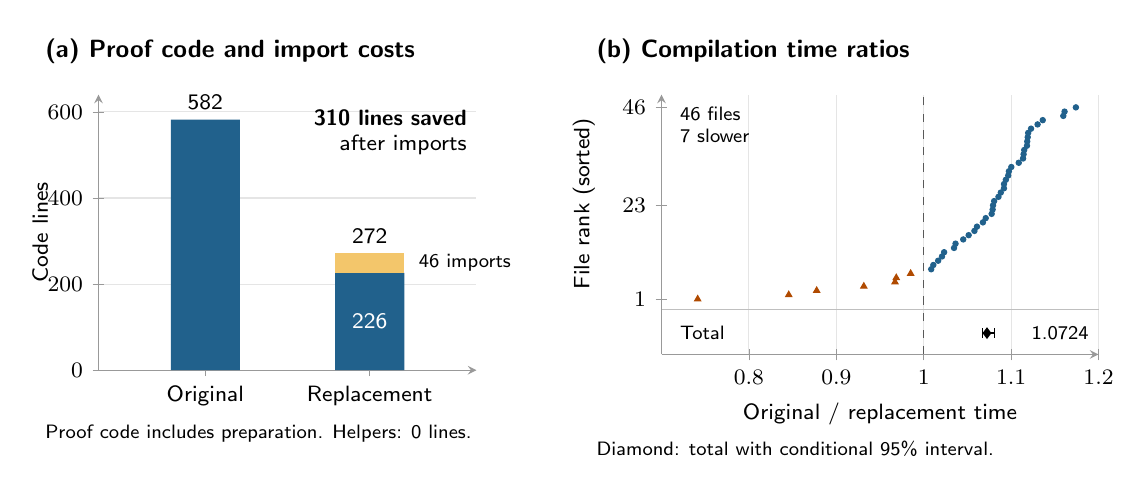
\begin{tikzpicture}[font=\sffamily\fontsize{8}{9}\selectfont]
\definecolor{proofblue}{HTML}{21618C}
\definecolor{importgold}{HTML}{F3C66B}
\definecolor{slowerorange}{HTML}{B04A00}
\path[use as bounding box] (0,0) rectangle (13.85,5.5);
\node[anchor=west,font=\sffamily\bfseries\fontsize{9}{10}\selectfont] at (0.1,5.2) {(a) Proof code and import costs};
\node[anchor=west,font=\sffamily\bfseries\fontsize{9}{10}\selectfont] at (7.1,5.2) {(b) Compilation time ratios};
\node[rotate=90] at (0.16,2.9) {Code lines};
\begin{axis}[
  at={(0.9cm,1.15cm)},anchor=south west,width=4.8cm,height=3.5cm,scale only axis,
  axis lines=left,axis line style={black!40},tick style={black!40},
  xmin=-0.65,xmax=1.65,ymin=0,ymax=640.2,
  xtick={0,1},xticklabels={Original,Replacement},ytick={0,200,400,600},
  ymajorgrids,grid style={black!10},clip=false,
  tick label style={font=\sffamily\fontsize{8}{9}\selectfont}]
\addplot[ybar,bar width=25pt,fill=proofblue,draw=none] coordinates {(0,582) (1,226)};

\draw[fill=importgold,draw=none] (axis cs:0.789,226) rectangle (axis cs:1.211,272);
\node[anchor=south] at (axis cs:0,582) {582};
\node[anchor=south] at (axis cs:1,272) {272};
\node[text=white] at (axis cs:1,113.0) {226};
\node[anchor=west,font=\sffamily\fontsize{7}{8}\selectfont] at (axis cs:1.24,249.0) {46 imports};
\node[anchor=north east,align=right] at (axis description cs:1,0.98) {\textbf{310 lines saved}\\after imports};
\end{axis}
\node[anchor=west,font=\sffamily\fontsize{7.5}{9}\selectfont] at (0.1,0.35) {Proof code includes preparation. Helpers: 0 lines.};
\begin{axis}[
  at={(8.05cm,1.35cm)},anchor=south west,width=5.55cm,height=3.3cm,scale only axis,
  axis lines=left,axis line style={black!40},tick style={black!40},
  xmin=0.7,xmax=1.2,ymin=-12,ymax=49,
  xtick={0.8,0.9,1,1.1,1.2},ytick={1,23,46},
  xlabel={Original / replacement time},xlabel style={at={(axis description cs:0.5,-0.15)}},
  ylabel={File rank (sorted)},ylabel style={at={(axis description cs:-0.13,0.58)}},
  xmajorgrids,grid style={black!10},clip=false,
  tick label style={font=\sffamily\fontsize{8}{9}\selectfont}]
\draw[black!65,dashed] (axis cs:1,-12) -- (axis cs:1,49);
\draw[black!25] (axis cs:0.7,-1.5) -- (axis cs:1.2,-1.5);
\addplot[only marks,mark=triangle*,mark size=1.25pt,slowerorange] coordinates {(0.741357139847,1) (0.845561253674,2) (0.877521284666,3) (0.931459768234,4) (0.967131323301,5) (0.968582783098,6) (0.98505414282,7)};
\addplot[only marks,mark=*,mark size=0.95pt,proofblue] coordinates {(1.00856453733,8) (1.01099255289,9) (1.01649580211,10) (1.02090096852,11) (1.02333594287,12) (1.0346804215,13) (1.03640469425,14) (1.04520147001,15) (1.05142627488,16) (1.0580151652,17) (1.06089700174,18) (1.06772484123,19) (1.07093454343,20) (1.07773042792,21) (1.07883408301,22) (1.07931550879,23) (1.08057159265,24) (1.08551994374,25) (1.08816690133,26) (1.09179498655,27) (1.09184631071,28) (1.09396082032,29) (1.09665843775,30) (1.09744802585,31) (1.10021960597,32) (1.10872359949,33) (1.11363838426,34) (1.11427219842,35) (1.11499865996,36) (1.11814366284,37) (1.1184259669,38) (1.11897770835,39) (1.11949922878,40) (1.12279439257,41) (1.13028220534,42) (1.13617423612,43) (1.15969500658,44) (1.16115009764,45) (1.17410502814,46)};
\draw[black,line width=0.8pt] (axis cs:1.06694154388,-7) -- (axis cs:1.08140985362,-7);
\draw[black] (axis cs:1.06694154388,-8.1) -- (axis cs:1.06694154388,-5.9);
\draw[black] (axis cs:1.08140985362,-8.1) -- (axis cs:1.08140985362,-5.9);
\addplot[only marks,mark=diamond*,mark size=1.8pt,black] coordinates {(1.07238729499,-7)};
\node[anchor=west,font=\sffamily\fontsize{7}{8}\selectfont] at (axis cs:0.71,-7) {Total};
\node[anchor=east,font=\sffamily\fontsize{7}{8}\selectfont] at (axis cs:1.2,-7) {1.0724};
\node[anchor=north west,align=left,font=\sffamily\fontsize{7}{8}\selectfont] at (axis description cs:0.02,0.99) {46 files\\7 slower};
\end{axis}
\node[anchor=west,font=\sffamily\fontsize{7.5}{9}\selectfont] at (7.1,0.15) {Diamond: total with conditional 95\% interval.};
\end{tikzpicture}

\caption{Source savings and compilation times for the verified local patch.
Replacement proof lines include preparation, with imports shown separately.
Each point is a file ratio of mean original to mean replacement time over 40 paired passes.
Triangles mark all 7 files with larger mean replacement times.
Ratios above one favor the replacement.
The diamond and bar show the full-pass ratio and its conditional paired 95\% interval over repeated timings.}
\label{fig:evaluation}
\end{figure}


One selected replacement changes an estimate inside the Strong Law proof from \CaseBefore{} to \CaseAfter{} code lines.
It keeps the finite sum bound and pointwise normalization, then uses \NA{} to combine the norm bounds.
The tactic does not prove the Strong Law itself.
Appendix~\ref{app:examples} gives the two source blocks and their provenance.

\paragraph{Compilation results.}
We froze the code, patch, sample count, and analysis before 40 confirmatory paired passes over all \PatchFiles{} affected files.
Dependencies were already built.
The run includes tactic search, imports, proof construction, kernel checking, serialization, and C generation.
It excludes native C object compilation and Lake dispatch.
Mean original and replacement pass times are \StudyOriginal{} and \StudyReplacement{} seconds.
The ratio is \StudyRatio{}, with conditional paired 95\% interval $[\StudyLower{},\StudyUpper{}]$.

The interval uses ten blocks of four paired passes and assumes independent, representative blocks.
The result includes all measured passes and the seven files with larger mean replacement times.
The predeclared criterion, an interval wholly above one, is met.

The variants use different native imports.
Thus the ratio does not isolate the tactic algorithm.
It applies to this workload on the recorded machine.
Power snapshots and uncontrolled background activity limit generalization.
Appendix~\ref{app:evaluation} gives calibration, runtime details, and inference assumptions.

\section{Related work and scope}
HOL Light has \texttt{NORM\_ARITH}, and Isabelle has the \texttt{norm} method \citep{hollightnorm,isabellenorm}.
Solovay, Arthan, and Harrison prove decidability results for universal normed-space formulas \citep{solovay2012}.
We do not claim the first decision procedure.

In Lean, \texttt{module} checks vector identities, and \texttt{linarith} combines scalar inequalities.
The \texttt{bound} tactic provides structural inequality automation.
Our tactic searches for decomposition constraints before these proof checks.
Its contribution is an AI-assisted implementation, a checked certificate design, and an evaluation against library proofs.

The artifact addresses a documented normed-space request.
The patch is local, with no mathlib acceptance claim.
We did not run a separate comparison against other Lean tactics.
The baseline is the existing library proofs, including their use of automation.
The selected patch is not a held-out test of tactic success.

The study does not compare models, measure autonomous coding ability, or estimate AI productivity.
The finite theorem gives no parser coverage result or practical runtime bound.
The census records incomplete extraction and untried observations, including original single-line proofs.
This case illustrates AI-assisted construction of a reusable proof tool whose outputs and library edits can be checked independently.
\label{main-end}

\clearpage
\bibliographystyle{plainnat}
\bibliography{references}
\clearpage
\appendix
\section{Full proof of the finite characterization}\label{app:proof}

Validity here quantifies over all real seminormed spaces and all assignments of vector and scalar atoms.
Formal atoms can be linearly dependent in an input.
The reduction records all recognized rational vector-equality assumptions.

Scalar atoms and unsupported vector subterms have independent interpretations in the abstraction.
A countermodel can ignore the internal operations of opaque expressions.
This is completeness for the abstraction.
Lean validates each proof for the concrete goal.

\subsection{Encoding vector equalities}
Represent the original atoms by the standard basis of $\R^d$.
Set $V=\R^d$ and represent each observed term by its rational coefficient vector.
For each recognized vector equality $u=v$, add the observed difference $e=u-v$ and the scalar constraint $n_e=0$.
In the original context, the equality proves this zero-norm fact in Lean.

A nonzero vector can have zero norm in an arbitrary seminormed space.
The necessary converse is only a model construction for scalar conclusions.
First realize all norm values on $V$.
Then construct the quotient by the zero subspace of that seminorm.
Each encoded difference then becomes zero.
The quotient preserves each observed norm value.

Thus the scalar encoding is exact for the stated implication problem.
This justifies the frontend's zero-norm encoding.
The frontend does not construct an explicit vector-space quotient.

Let $U\subseteq V$ be the span of the observed vectors $v_1,\ldots,v_m$.
All constructions start on $U$.
The construction includes repeated vectors, opposite vectors, and zero vectors.

\begin{lemma}[Vertices and finite enumeration]\label{lem:vertices}
Let $M\in\Q^{r\times n}$ and $b\in\R^r$.
For $P=\{z\in\R^n_{\ge0}:Mz=b\}$, a feasible point is a vertex exactly when its positive-support columns are independent.
There are a finite number of vertices.
If $b\in\Q^r$, all vertices are rational.
If $P$ is nonempty and a nonnegative linear cost is bounded below on it, a minimum occurs at a vertex.
\end{lemma}
\begin{proof}
Suppose the support columns of a feasible $z$ are dependent.
Select a nonzero vector $h$ with support there and $Mh=0$.
For a sufficiently small $\epsilon>0$, the points $z+\epsilon h$ and $z-\epsilon h$ are nonnegative.
They are distinct feasible points with midpoint $z$.
Thus $z$ is not a vertex.

Suppose the support columns are independent.
If $z=(a+b)/2$ with feasible $a,b$, each zero coordinate of $z$ is zero in $a$ and $b$.
The difference $a-b$ thus has support on the independent columns.
Because $M(a-b)=0$, we get $a=b=z$.
This proves the vertex characterization.

Each independent support determines at most one solution.
There are a finite number of supports.
Thus there are a finite number of vertices.
When $b$ is rational, exact rational elimination gives rational coordinates for each such solution.

For the existence of an optimal vertex, write the cost as $w^Tz$ with $w\ge0$.
Let $z$ be a feasible point with dependent support.
Select $h$ as above.
If $h$ has the two signs, select the direction with nonpositive cost change.
Move to the first coordinate boundary in that direction.
This preserves feasibility, does not increase the cost, and decreases the support.

If $h$ has only one sign, select it nonnegative.
Move in direction $-h$.
Its cost change is nonpositive because $w\ge0$.
Again the move stops at a coordinate boundary.

Do this step again to get a feasible vertex with cost no greater than that of $z$.
The finite vertex set is nonempty and has a least-cost element.
Each feasible point has cost no less than the minimum.
Thus the vertex attains the infimum over $P$.
\end{proof}

The proof's last claim applies to each nonnegative cost used here.
Strictly positive norm values and a bounded feasible polyhedron are not necessary.
For $M=[A,-A]$, the positive support cannot contain the two copies of a nonzero column.
The signed solution on an independent unsigned subset thus represents the same vertex data.
Zero columns add no positive coordinate at a vertex.
The all-zero point is a vertex when $b=0$.

\begin{lemma}[Necessity]\label{lem:necessary}
Each vector assignment that satisfies the recognized equalities has norm values that satisfy \eqref{eq:constraints}.
\end{lemma}
\begin{proof}
The assignment induces a seminorm on $V$ through a linear map.
Seminorms are nonnegative, and the encoded equality differences have norm zero.
For $z\in P_i$, the equality $[A,-A]z=v_i$ gives
\[
 v_i=\sum_j z_jv_j+\sum_j z_{m+j}(-v_j).
\]
Subadditivity, absolute homogeneity, and $z\ge0$ give
$\norm{v_i}\le\sum_j(z_j+z_{m+j})\norm{v_j}$.
This holds for all feasible points.
Thus it holds for each vertex.
\end{proof}

\begin{lemma}[Realization]\label{lem:realization}
Suppose nonnegative $n_1,\ldots,n_m$ satisfy \eqref{eq:constraints}.
There is a seminorm $p$ on $V$ with $p(v_i)=n_i$ for each $i$.
\end{lemma}
\begin{proof}
For $u\in U$, the feasible set in \eqref{eq:gauge} is nonempty.
A real linear representation of $u$ in the columns of $A$ splits into positive and negative parts.
Its cost is nonnegative.
Lemma~\ref{lem:vertices} shows that the minimum defining $p(u)$ exists and is finite.
The zero representation gives $p(0)=0$.

If $z$ represents $u$, an exchange of its first and last $m$ coordinates represents $-u$ with equal cost.
Thus $p(-u)=p(u)$.
For $\lambda>0$, multiplication by $\lambda$ gives a bijection between the representations of $u$ and $\lambda u$.
Costs multiply by $\lambda$.
Thus $p(\lambda u)=\lambda p(u)$.
Symmetry and the zero case give $p(\lambda u)=|\lambda|p(u)$ for each real $\lambda$.

If $z$ and $z'$ minimize the costs of $u$ and $u'$, then $z+z'$ represents $u+u'$.
Thus $p(u+u')\le p(u)+p(u')$.
These facts prove that $p$ is a seminorm on $U$.

The representation of $v_i$ by one positive column has cost $n_i$.
Thus $p(v_i)\le n_i$.
By Lemma~\ref{lem:vertices}, an optimal representation of $v_i$ is a vertex of $P_i$.
Its constraint in \eqref{eq:constraints} gives $n_i\le p(v_i)$.
Thus $p(v_i)=n_i$.

Select a real linear complement $W$ with $V=U\oplus W$.
Define $\widetilde p(u+w)=p(u)$ for $u\in U$ and $w\in W$.
The uniqueness of the direct-sum decomposition makes this well-defined.
Linearity of the projection onto $U$ preserves homogeneity and subadditivity.
Thus $\widetilde p$ is the stated seminorm on $V$.
\end{proof}

\begin{proof}[Proof of Theorem~\ref{thm:complete}]
Lemma~\ref{lem:necessary} proves necessity.
Each vector equality also gives its recorded zero-norm constraint.
For sufficiency, apply Lemma~\ref{lem:realization} on $V=\R^d$.
Let $K=\{v:p(v)=0\}$ be the kernel of this seminorm.
Homogeneity and subadditivity make $K$ a vector subspace, and $p$ induces a norm on $V/K$.
Assign each formal atom its basis class in that quotient.

Each encoded equality difference belongs to $K$.
Thus the assignment satisfies each vector equality.
The quotient preserves $p(v_i)=n_i$ for each observed term.
It is a normed space and thus also a seminormed space.

Replace each observed norm by a real variable $n_i$.
Conjoin \eqref{eq:constraints}, the scalar assumptions, and the negation of the proposed conclusion.
The resulting problem is rational linear feasibility for a finite system with strict and weak comparisons.
A feasible solution extends to a seminormed-space counterexample by the realization lemma.

By necessity, a counterexample gives a feasible solution.
Thus infeasibility is equivalent to validity of the implication.
An equality conclusion is the conjunction of two weak inequalities, or equivalently its negation splits into two strict branches.
Exact linear arithmetic decides each finite branch.
This proves mathematical completeness of the reference reduction.
\end{proof}

The intermediate construction can have a nontrivial seminorm kernel.
Its quotient is a normed-space model with the same scalar norm values and the necessary vector equalities.
This observation is valid only for a grammar without vector-disequality assumptions or vector-equality conclusions.
For multiple vector types, apply the construction to each type and combine their scalar constraints.
Different spaces share scalar values but not vector identities.

\subsection{Removing the target from the source set}
The full polyhedron in \eqref{eq:polyhedron} always contains the trivial single-column representation.
An implementation can exclude $v_i$ during the generation of nontrivial bounds on $n_i$.
This optimization preserves the finite characterization.

Use a representation $v_i=c_iv_i+\sum_{j\ne i}c_jv_j$.
If $|c_i|\ge1$, nonnegativity implies its norm inequality.
If $|c_i|<1$, then $c_i\ne1$ and
\[
 v_i=\sum_{j\ne i}\frac{c_j}{1-c_i}v_j.
\]
The target-free constraints bound $n_i$ by the minimum cost of such representations.
Lemma~\ref{lem:vertices} reduces the minimum to their vertices.
Because $|1-c_i|\ge1-|c_i|$, this bound implies
\[
 (1-|c_i|)n_i\le\sum_{j\ne i}|c_j|n_j,
\]
which is the original self-containing inequality.

If no target-free representation exists, no such $|c_i|<1$ representation exists.
The trivial inequalities add no restriction.

\subsection{Strict scalar comparisons}
Strict comparisons do not use approximate arithmetic.
One exact feasibility construction replaces all strict rows $a_r^Ty<b_r$ by
$a_r^Ty\le b_r-\delta$, adds $0\le\delta\le1$, and maximizes $\delta$.
The original finite system is feasible exactly when the weak rows are feasible and this bounded linear program has a positive optimum.

For a feasible strict system, its finite set of positive gaps has a minimum that gives such a $\delta$.
The converse follows directly from $\delta>0$.
If there are no strict rows, weak feasibility suffices.
This is one reference argument.
It does not specify the Lean backend reduction.

\section{Checked examples and source provenance}\label{app:examples}
The release records a successful source compilation for all marked blocks. This build checked their saved hashes.

The generated manifest records source hashes and marker ranges.
The paper does not change the imported blocks.

\subsection{The community request and rational averaging}
The main-text source quote is from \sourcepath{NormArithTest/Tactic.lean} at the measured source snapshot.
The build extracts it from the validated archive and records its source hash and line range.
A separate fresh check of the full test module includes this exact inequality.
It is additional to the six archived paper examples.

The averaging example finds $x=\frac12(x+y)+\frac12(x-y)$ from two local bounds.
Here $E$ is a real seminormed space.
It demonstrates automatic bound selection and fractional coefficients.
\VerbatimInput{generated/hidden.lean}


\subsection{Quantified bounds and generic metric chains}
The quantified example specializes the local hypothesis at two observed arguments.
It normalizes ball membership, proves the radius premises with restricted scalar arithmetic, and checks the cancellation identity.
It does not search arbitrary values of the quantified variable.
\VerbatimInput{generated/quantified.lean}


The metric example uses no addition or scalar multiplication on its points.
Here $X$ is a pseudometric space.
Symmetry reverses the second bound.
Triangle constraints and scalar arithmetic complete the chain.
\VerbatimInput{generated/metric.lean}


The specialization limits are 12 templates, 12 binders per template, 32 observed vectors, 32 new bounds, and 128 candidate attempts.
Each attempt checks at most eight additive patterns of depth at most eight.
Premise construction has depth four.
Norm alias filtering has depth eight and a 256-node budget.
When inspection is incomplete, the tactic excludes that expression.

The fixed rewrite set has rules for distances, balls, closed balls, the four bounded interval types, and membership in sets defined by predicates.
This is not an unrestricted simplifier or quantified decision procedure.
The metric path collects at most eight points in total.
These limits give partial coverage, without changing Theorem~\ref{thm:complete}.

\subsection{Strict and reverse-triangle reasoning}
The reverse-triangle estimate compares a difference of norms with the norm of a vector difference.
The finite constraints supply a triangle bound.
Scalar arithmetic rearranges it.
The comparison grammar also includes strict scalar relations.
\VerbatimInput{generated/reverse.lean}


\subsection{A checked boundary and the additive extension}
Products of norms are not in the declared scalar grammar.
This statement is true.
In the negative tactic test, \NA{} must reject that unsupported goal.
A multiplication lemma completes the Lean proof.
This records an unsupported input.
It is not a counterexample to the theorem or a timeout.
\VerbatimInput{generated/boundary.lean}


For $n\in\mathbb N$, the additive groups give $\norm{n\mathbin{\bullet}x}\le n\norm{x}$.
This does not give real homogeneity.
For example, the discrete norm on $\mathbb Z$ is zero at zero and one at all nonzero inputs.
At $x=1$, $\norm{x}$ and $\norm{2x}$ are one.
Thus $\norm{2x}\le1$ does not imply $\norm{x}\le1/2$ in that class.
Do not use the real-space certificate in this class.

\subsection{The selected composed patch example}
\begingroup\raggedright
The selected entry is \texttt{manual-strong-law-sums}. Its source is \sourcepath{Mathlib/Probability/StrongLaw.lean}, lines 760--780. Its declaration is \sourcepath{ProbabilityTheory.strong_law_ae_of_measurable}. The final combined source check includes this entry.

\par\endgroup
The source replacement changes one estimate inside the Strong Law argument.
The preparation uses the existing finite sum bound, norm homogeneity, and the sum triangle inequality.
It distributes subtraction and scalar multiplication before the tactic combines the bounds.
It preserves the full theorem statement and its assumptions.
The tactic does not prove the convergence hypotheses or the Strong Law.
\paragraph{Original source block.}
\VerbatimInput{generated/census-example-original.lean}
\paragraph{Replacement source block.}
\VerbatimInput{generated/census-example-replacement.lean}

\subsection{An operator estimate}
The source example is the candidate \texttt{fderiv-telescope} at the pinned mathlib revision.
The build extracts the original and replacement blocks from the recorded manifest and pinned source.
The generation code validates their source hashes.
This checked example abstracts the shared bound and renames the four operator values.
It generalizes the proof shape.
It does not give the literal mathlib source.

Here $E$ is an additive group.
\VerbatimInput{generated/mathlib.lean}

\paragraph{Original source block.}
\VerbatimInput{generated/mathlib-original.lean}
\paragraph{Replacement source block.}
\VerbatimInput{generated/mathlib-replacement.lean}

\section{Evaluation protocol and artifact status}\label{app:evaluation}
The study uses Lean \texttt{4.36.0-rc1} and this mathlib revision:
\begin{quote}\small\texttt{2f3c7c8a8949b04a32f9303f59163acffb766996}\end{quote}

\paragraph{Implementation paths.}
The frontend rewrites distances, collects norm arguments, and encodes recognized vector equalities as checked zero-norm facts.
It tries structural bounds and short decompositions before the finite reference family.
The reference search records the status of its independent-support enumeration: complete or resource-exhausted.
Its default limits are 10,000 support systems and 10,000 retained results.
The support-attempt count excludes the initial full-system rank test.

The public interface also keeps a sound upper-bound extension with an opaque scalar right side.
This path handles bounds that the affine scalar grammar excludes.
It has no stated completeness guarantee.
The additive-group path also has partial coverage.
Added signed integer proposals can succeed where rational averaging is unavailable.
Each path that succeeds constructs a Lean-validated certificate.

Certificate identities must complete elaboration and synthesis before acceptance.
Definitional vector aliases use checked normalization.
Elaboration recovery does not replace a failed proof by \texttt{sorry}.
The scalar backend uses exact proof construction at matching transparency.

\paragraph{Composed evidence.}
The historical full census gives the pinned source universe and its retained coverage gaps.
The targeted follow-up gives a separate source subset, protocol, outcome ledger, and isolated proposals.
The patch contains 50 census-generated replacements and 37 replacements composed outside the census.

The selector combines census-generated replacements with replacements composed outside the census.
Replacements composed outside the census can supply explicit facts or add preparation.
Artificial intelligence (AI) coding agents assisted their development.
The accounting counts all added preparation.

The selector recomputes disjoint source edits and checks original declaration body observations.
Final combined compilation, implementation snapshots, the frozen patch, and the new timing run form a separate chain.
The historical full census tactic implementation does not supply a speed result for this chain.

\paragraph{Line accounting.}
The accounting counts nonblank, noncomment lines of proof code in the formatted source.
It counts preparation in each replacement and each shared helper declaration one time.

The report counts imports and includes them in the net figure.
The savings describe only the deterministic nonoverlapping combined patch.
The report also counts the tactic implementation and census infrastructure.
This count does not show a net reduction in the library's total source size.

\paragraph{Semantic census.}
The census uses the sorted tracked Lean sources in \texttt{Mathlib/} at the pinned revision.
The census includes tactic observations and expected-type information from term proofs.
The extractor waits for finalized elaboration data.
It records original source spans, declarations, normalized goals, local facts, eligibility, attempts, and per-file completion.
The ledger gives explicit classes to macro-generated, overlapping, abandoned, or uneditable observations.

A checked replay proposal is not a verified source replacement.
The full source patch compiled with all selected replacements together.
The census denominator includes extraction failures and exhausted files.

The full census uses four workers.
The targeted follow-up uses three.
Each worker uses one Lean thread and a 600-second file limit.
Each worker has a 4096 MB memory limit.

A resource-failure retry uses one worker, an 1800-second file limit, and 8192 MB.
The per-goal limits are 200000 heartbeats and 2000 milliseconds.
The scan makes no added preparation and does not try original single-line proofs.

An eligible observation must have an editable source span and a closed local context.
Unlocated or unresolved nodes are coverage gaps even in files with complete extraction.
Their counters are not counts of distinct unsupported goals.

The census has 99 known eligible observations without a recorded outcome because a file did not complete. Failed files can also have goals that extraction did not record. Counters from final file records do not count all known observations. The follow-up has 0 known eligible observations without terminal outcomes.
\begin{table}[!htbp]\centering\small
\caption{Historical full census, targeted follow-up, and composed verified patch. The datasets are separate. Proof counts include preparation, helpers, and imports.}
\begin{tabular}{lr}\toprule
Measure & Value\\\midrule
Tracked files processed & 8637\\
Files with complete extraction & 8610\\
Files with incomplete outcomes & 27\\
Known eligible observations & 20628\\
Isolated checked proposals & 40\\
Targeted follow-up files processed & 885\\
Follow-up complete / incomplete files & 875 / 10\\
Follow-up isolated checked proposals & 158\\
Compiled proof spans / affected files & 87 / 46\\
Original / replacement proof lines & 582 / 226\\
Added helper / import lines & 0 / 46\\
Net lines saved after helpers and imports & 310\\
Ratio of mean compilation times & 1.0724\\
Paired 95\% interval & [1.0669, 1.0814]\\
\bottomrule\end{tabular}\end{table}

\begin{table}[!htbp]\centering\small
\caption{Final file outcomes and outcomes for known eligible observations. The counters use final file records and exclude files without those records. Known observations without outcomes are not tactic failures.}
\begin{tabular}{lr}\toprule
Recorded outcome & Count\\\midrule
augmented\_elaboration\_failed & 4\\
complete & 8610\\
file\_timeout & 1\\
original\_elaboration\_failed & 5\\
partial\_extraction & 14\\
process\_failed & 3\\
attempt: augmented\_elaboration\_failed & 15\\
attempt: context\_unmatched & 4\\
attempt: failed & 2753\\
attempt: import\_cycle & 54\\
attempt: no\_line\_saving\_untried & 17663\\
attempt: success & 40\\
Unknown due to incomplete files & 99\\
final file record: duplicate & 19598\\
final file record: eligible & 20385\\
final file record: errors & 54\\
final file record: normGoals & 122441\\
final file record: outsideBody & 448\\
final file record: proofNodes & 5164910\\
final file record: synthetic & 0\\
final file record: tacticNodes & 5945347\\
final file record: termNodes & 34310511\\
final file record: unlocatedNodes & 12037137\\
final file record: unresolved & 12445\\
\bottomrule\end{tabular}\end{table}

\begin{table}[ht]\centering\small
\caption{Observed fragments and their recorded outcomes. These counts are not combined patch savings.}
\begin{tabular}{lr}\toprule
Fragment and outcome & Count\\\midrule
observed: additive\_group\_extension & 12306\\
observed: core & 14628\\
observed: outside\_fragment & 90124\\
observed: upper\_bound\_extension & 6215\\
eligible: additive\_group\_extension & 8139\\
eligible: core & 8989\\
eligible: upper\_bound\_extension & 3500\\
additive\_group\_extension: augmented\_elaboration\_failed & 8\\
additive\_group\_extension: context\_unmatched & 2\\
additive\_group\_extension: failed & 958\\
additive\_group\_extension: import\_cycle & 30\\
additive\_group\_extension: no\_line\_saving\_untried & 7094\\
additive\_group\_extension: success & 15\\
core: failed & 1077\\
core: import\_cycle & 2\\
core: no\_line\_saving\_untried & 7887\\
core: success & 23\\
upper\_bound\_extension: augmented\_elaboration\_failed & 7\\
upper\_bound\_extension: context\_unmatched & 2\\
upper\_bound\_extension: failed & 718\\
upper\_bound\_extension: import\_cycle & 22\\
upper\_bound\_extension: no\_line\_saving\_untried & 2682\\
upper\_bound\_extension: success & 2\\
\bottomrule\end{tabular}\end{table}

\begin{table}[!htbp]\centering\small
\caption{Targeted follow-up outcomes. This subset does not give a new full-universe census.}
\begin{tabular}{lr}\toprule
Recorded outcome & Count\\\midrule
file: augmented\_elaboration\_failed & 8\\
file: complete & 875\\
file: partial\_extraction & 2\\
attempt: augmented\_elaboration\_failed & 42\\
attempt: context\_unmatched & 8\\
attempt: failed & 6475\\
attempt: goal\_timeout & 38\\
attempt: import\_cycle & 192\\
attempt: no\_line\_saving\_untried & 20742\\
attempt: success & 158\\
Unknown due to incomplete files & 0\\
\bottomrule\end{tabular}\end{table}

\begin{table}[ht]\centering\small
\caption{Known eligible follow-up observations by original goal fragment. Isolated proposals and composed patch savings are separate.}
\begin{tabular}{lr}\toprule
Fragment & Count\\\midrule
additive\_group\_extension & 8936\\
core & 10362\\
metric\_extension & 4065\\
upper\_bound\_extension & 4292\\
\bottomrule\end{tabular}\end{table}

\begin{table}[!htbp]\centering\small
\caption{Deterministic selection outcomes before source verification. The selection ledger records the causes. The verified combined patch gives the proof savings.}
\begin{tabular}{lr}\toprule
Selection outcome & Count\\\midrule
duplicate\_replacement & 23\\
import\_cost\_offsets\_savings & 29\\
no\_line\_saving & 8\\
overlap & 61\\
selected & 87\\
\bottomrule\end{tabular}\end{table}

\begin{table}[!htbp]\centering\small
\caption{Implementation code has a separate cost from the proposed mathlib proof savings. These totals do not show a reduction in total repository size.}
\begin{tabular}{lr}\toprule
Component & Code lines\\\midrule
Tactic implementation & 850\\
Census infrastructure & 470\\
\bottomrule\end{tabular}\end{table}


\FloatBarrier

\paragraph{Historical source format correction.}
An earlier patch had a proof line longer than mathlib's source-style limit.
The format correction removed that file's net line saving.
The historical 41-line patch then passed new source verification, calibration, and confirmatory timing.
The historical timing runs do not give an estimate for the expanded patch.

\paragraph{Confirmatory timing.}
We used paired passes over exactly the same affected files.
Dependencies were built before measurement.
Each pass emitted fresh compiler outputs.
The run alternated the two variant sequences.
For original totals $O_1,\ldots,O_N$ and replacement totals $R_1,\ldots,R_N$, the primary ratio is
\[
 S=\frac{\frac1N\sum_tO_t}{\frac1N\sum_tR_t}.
\]

We grouped the $N$ paired passes in sequence into $K=N/b$ blocks of the calibrated even length $b$.
The blocks have equal length and do not overlap.
Each block includes the two variants and all affected files.
For each replicate, the bootstrap selects $K$ full blocks with replacement.
It keeps all observations of each selected block together.
The even block length gives equal counts of the two variant sequences.

The sequences are original then replacement, and replacement then original.
There are $K$ sampling units.

The method uses the bias-corrected and accelerated (BCa) probability transformation \citep{efron1987}.
For acceleration, the jackknife removes one full block at a time \citep{diciccioefron1996}.
The implementation gives half weight to bias-correction ties.
It uses linear interpolation for empirical quantiles.

A bootstrap method has model assumptions \citep{fieldwelsh2007}.
The interval uses a model with independent, representative blocks for the recorded timing conditions.
The calibration uses pilot diagnostics to select the block length.
These diagnostics do not prove the assumptions.

Timing conditions can change over time.
The interval is for runs of this fixed workload on the recorded machine.
It does not give a result for other hardware or mathlib revisions.
The paper gives no coverage theorem for arbitrary timing dependence.

We fixed the sample count, block length, seed, bootstrap count, and stopping rule before the confirmatory run.
The success criterion was a full paired 95\% interval for $S$ greater than one.

The block-length review used a separate 24-pair pilot. It excluded absolute times, average speed levels, confidence intervals, and significance. It selected 4 pairs for each block before the confirmatory run. There were 6 pilot blocks at this block length. These diagnostics do not prove block independence.
\begin{table}[ht]\centering\small
\caption{Blinded pilot diagnostics for the frozen block-length decision. The review used serial, drift, and order metrics. These diagnostics do not prove independence.}
\begin{tabular}{lr}\toprule
Diagnostic & Value\\\midrule
Measured pilot pairs & 24\\
Duration correlation at lag 1 (original / patch) & 0.125 / 0.173\\
Duration correlation at lag 2 (original / patch) & 0.011 / -0.269\\
4-pair duration correlation at lag one & 0.218 / -0.260\\
8-pair duration correlation at lag one & -0.182 / -0.391\\
Half-run duration change (\%) & -2.469 / -0.703\\
Change in mean log ratio & -0.017\\
AB minus BA relative duration (\%) & 0.861 / 0.266\\
AB minus BA mean log ratio & 0.005\\
4-pair log-ratio correlations at lags 1--3 & 0.323 / -0.051 / -0.252\\
Pilot / confirmatory blocks & 6 / 10\\
\bottomrule\end{tabular}\end{table}


\FloatBarrier

The analysis kept slower files, failed attempts, and measured passes.
Timeouts or incomplete variants prevent a complete-compilation claim for those variants.
The table separates setup processes from unmeasured dependency and native builds.
Search-based compilation is the primary measurement.
The study does not give timing results for explicit certificate replay.

The confirmatory run uses 10 blocks of 4 paired passes. It uses 10000 bootstrap samples with seed 20261020. The ratio of mean full-pass times is 1.0724. The conditional paired 95\% interval is [1.0669, 1.0814].

The predeclared speed criterion is met. The analysis includes all affected files and measured passes.

Second-half mean times changed by +4.26\% for original and +5.14\% for replacement relative to the first half. The interval remains conditional on independent, representative timing blocks.
{\small
\begin{longtable}{p{0.61\linewidth}rrr}
\caption{Confirmatory means in seconds for each affected file. The ratio is original time divided by replacement time. The analysis includes slower files.}\\\toprule
Affected file & Original & Patch & Ratio\\\midrule
\endfirsthead
Affected file & Original & Patch & Ratio\\\midrule\endhead
\nolinkurl{Mathlib/Analysis/Analytic/Basic.lean} & 5.114 & 4.555 & 1.1228\\
\nolinkurl{Mathlib/Analysis/Asymptotics/AsymptoticEquivalent.lean} & 1.906 & 1.711 & 1.1143\\
\nolinkurl{Mathlib/Analysis/Asymptotics/SpecificAsymptotics.lean} & 1.659 & 1.538 & 1.0788\\
\nolinkurl{Mathlib/Analysis/Calculus/BumpFunction/FiniteDimension.lean} & 3.036 & 2.715 & 1.1181\\
\nolinkurl{Mathlib/Analysis/Calculus/FDeriv/Basic.lean} & 3.283 & 2.890 & 1.1362\\
\nolinkurl{Mathlib/Analysis/Calculus/FDeriv/Measurable.lean} & 4.400 & 4.185 & 1.0514\\
\nolinkurl{Mathlib/Analysis/Complex/OpenMapping.lean} & 2.170 & 2.014 & 1.0777\\
\nolinkurl{Mathlib/Analysis/Convex/Uniform.lean} & 1.288 & 1.738 & 0.7414\\
\nolinkurl{Mathlib/Analysis/Fourier/RiemannLebesgueLemma.lean} & 2.260 & 2.180 & 1.0364\\
\nolinkurl{Mathlib/Analysis/LocallyConvex/Polar.lean} & 1.726 & 1.651 & 1.0452\\
\nolinkurl{Mathlib/Analysis/Normed/Algebra/Spectrum.lean} & 4.085 & 3.723 & 1.0974\\
\nolinkurl{Mathlib/Analysis/Normed/Algebra/Unitization.lean} & 2.629 & 2.586 & 1.0165\\
\nolinkurl{Mathlib/Analysis/Normed/Field/Approximation.lean} & 1.585 & 1.571 & 1.0086\\
\nolinkurl{Mathlib/Analysis/Normed/Group/ControlledClosure.lean} & 1.235 & 1.275 & 0.9686\\
\nolinkurl{Mathlib/Analysis/Normed/Module/MStructure.lean} & 1.549 & 1.663 & 0.9315\\
\nolinkurl{Mathlib/Analysis/Normed/Module/Multilinear/Basic.lean} & 8.264 & 7.739 & 1.0677\\
\nolinkurl{Mathlib/Analysis/Normed/Operator/Banach.lean} & 3.972 & 3.881 & 1.0233\\
\nolinkurl{Mathlib/Analysis/Normed/Order/Lattice.lean} & 1.320 & 1.340 & 0.9851\\
\nolinkurl{Mathlib/Analysis/SpecialFunctions/Complex/LogBounds.lean} & 3.207 & 2.995 & 1.0709\\
\nolinkurl{Mathlib/Analysis/SpecialFunctions/Elliptic/Weierstrass.lean} & 9.987 & 9.200 & 1.0855\\
\nolinkurl{Mathlib/Analysis/SpecialFunctions/Exp.lean} & 1.949 & 1.678 & 1.1612\\
\nolinkurl{Mathlib/Analysis/SpecialFunctions/FrullaniIntegral.lean} & 1.978 & 1.831 & 1.0806\\
\nolinkurl{Mathlib/Computability/AkraBazzi/GrowsPolynomially.lean} & 3.483 & 3.128 & 1.1136\\
\nolinkurl{Mathlib/MeasureTheory/Constructions/HaarToSphere.lean} & 2.572 & 2.544 & 1.0110\\
\nolinkurl{Mathlib/MeasureTheory/Covering/BesicovitchVectorSpace.lean} & 2.594 & 2.452 & 1.0580\\
\nolinkurl{Mathlib/MeasureTheory/Function/AEEqOfIntegral.lean} & 1.933 & 1.771 & 1.0918\\
\nolinkurl{Mathlib/MeasureTheory/Function/ConvergenceInDistribution.lean} & 2.140 & 1.951 & 1.0967\\
\nolinkurl{Mathlib/MeasureTheory/Function/Jacobian.lean} & 4.147 & 3.669 & 1.1303\\
\nolinkurl{Mathlib/MeasureTheory/Function/L1Space/Integrable.lean} & 4.264 & 3.632 & 1.1741\\
\nolinkurl{Mathlib/MeasureTheory/Integral/DominatedConvergence.lean} & 2.912 & 2.511 & 1.1597\\
\nolinkurl{Mathlib/MeasureTheory/Integral/FinMeasAdditive.lean} & 3.182 & 2.854 & 1.1150\\
\nolinkurl{Mathlib/MeasureTheory/Integral/PeakFunction.lean} & 2.574 & 2.353 & 1.0940\\
\nolinkurl{Mathlib/MeasureTheory/Measure/IntegralCharFun.lean} & 1.766 & 1.618 & 1.0918\\
\nolinkurl{Mathlib/MeasureTheory/Measure/SeparableMeasure.lean} & 2.237 & 2.191 & 1.0209\\
\nolinkurl{Mathlib/NumberTheory/Padics/PadicNumbers.lean} & 3.785 & 3.381 & 1.1195\\
\nolinkurl{Mathlib/Probability/StrongLaw.lean} & 3.850 & 3.441 & 1.1190\\
\nolinkurl{Mathlib/Topology/Bornology/BoundedOperation.lean} & 1.279 & 1.206 & 1.0609\\
\nolinkurl{Mathlib/Topology/ContinuousMap/Bounded/ArzelaAscoli.lean} & 1.117 & 1.273 & 0.8775\\
\nolinkurl{Mathlib/Topology/ContinuousMap/Bounded/Basic.lean} & 2.578 & 2.325 & 1.1087\\
\nolinkurl{Mathlib/Topology/ContinuousMap/Bounded/Normed.lean} & 3.469 & 3.188 & 1.0882\\
\nolinkurl{Mathlib/Topology/MetricSpace/Gluing.lean} & 1.804 & 1.744 & 1.0347\\
\nolinkurl{Mathlib/Topology/MetricSpace/GromovHausdorff.lean} & 3.251 & 3.012 & 1.0793\\
\nolinkurl{Mathlib/Topology/MetricSpace/GromovHausdorffRealized.lean} & 2.208 & 2.007 & 1.1002\\
\nolinkurl{Mathlib/Topology/MetricSpace/Kuratowski.lean} & 1.302 & 1.346 & 0.9671\\
\nolinkurl{Mathlib/Topology/MetricSpace/PiNat.lean} & 2.825 & 2.526 & 1.1184\\
\nolinkurl{Mathlib/Topology/MetricSpace/Polish.lean} & 1.313 & 1.552 & 0.8456\\
Total & 131.188 & 122.333 & 1.0724\\
\bottomrule\end{longtable}}

\begin{table}[ht]\centering\small
\caption{Recorded setup costs outside measured compilation times. These costs do not include a full build without dependency artifacts.}
\begin{tabular}{lr}\toprule
Setup measurement & Seconds\\\midrule
Recorded setup processes & 296.029\\
Separate tactic rebuild & Not measured\\
Build without dependency/native artifacts & Not measured\\
\bottomrule\end{tabular}\end{table}


\FloatBarrier

The variants use native plugin configurations from their recorded headers.
The replacement imports can load Mathlib and tactic native libraries for unchanged tactics.
The ratio includes these import configurations.
It does not prove an algorithmic improvement.
A separate algorithm comparison must use the same runtime and imports.

The study did not measure a full build without dependency or native-library artifacts.
The numerical runtime was Python 3.15.0.
The recorded runtime and numerical rules define the exact bootstrap hashes.

\paragraph{Recorded hardware.}
The hardware profile records an Apple M4 Max MacBook Pro with 36 GiB of memory.
The logical processor count is 14.
The recorded operating system is macOS 26.7.1.

Snapshots before and after the study show the source label \texttt{AC Power}.
They show low-power mode off and sleep disabled.
The battery snapshots show 80\% before the study and 41\% after it.
The later snapshot also shows battery discharging.

Queries for thermal status failed.
These snapshots do not show continuous power or thermal stability.
The study did not control background activity.

\section{AI development provenance and limits}\label{app:development}
The motivating request is the May 2020 Lean community discussion of norm decompositions \citep{leanrequest2020}.
The repository test module contains the same inequality, with the decomposition implicit in the tactic call.
The averaging example exercises rational coefficients beyond that motivating example.
These examples address the normed-space decomposition request.
They do not establish community endorsement or solve the later normed-algebra request.

The project development guide records that ChatGPT generated the starter.
The expansion commit records \texttt{Assisted-by: Codex:GPT-6}.
The repository also records AI assistance in developing and reviewing library source edits.
These records support an AI-assisted development account, without assigning every source line to a particular tool.
The \href{https://github.com/TomasOrtega/norm-arith/tree/0f9b637e6f3f385e8ffa7c8a6135beb0e9c6fdc2}{measured source snapshot} contains the development guide, code, tests, and evaluation artifacts.

\paragraph{Recorded development steps.}
The \href{https://github.com/TomasOrtega/norm-arith/commit/e5b88e1}{starter commit} contains the initial code and its ChatGPT disclosure.
The design records first specify \href{https://github.com/TomasOrtega/norm-arith/blob/0f9b637e6f3f385e8ffa7c8a6135beb0e9c6fdc2/docs/adr/0002-initial-tactic-fragment.md}{explicit upper bounds}, then adopt \href{https://github.com/TomasOrtega/norm-arith/blob/0f9b637e6f3f385e8ffa7c8a6135beb0e9c6fdc2/docs/adr/0004-automatic-bound-discovery.md}{automatic selection} while preserving explicit fact control.
A \href{https://github.com/TomasOrtega/norm-arith/blob/0f9b637e6f3f385e8ffa7c8a6135beb0e9c6fdc2/docs/adr/0008-normalized-core-and-shared-certificates.md}{later decision} puts optimized paths and the finite reference search behind the same certificate interface.
They record project decisions without attributing every decision to an agent or a human.

The \href{https://github.com/TomasOrtega/norm-arith/tree/0f9b637e6f3f385e8ffa7c8a6135beb0e9c6fdc2/artifacts/expansion/next/production-regressions}{regression archive} records failures for function aliases and set-membership bounds, followed by a complete successful build.
For example, expressions written with \sourcepath{Function.uncurry} failed during certificate identity checking.
The correction used immediate checked identity synthesis, matching normalization settings, and restricted fact selection.
The archive binds the failed logs, revised tactic, tests, and successful build with source hashes.
The tests include positive examples and rejection of omitted norm premises.
This is one documented repair, not a complete record of development failures.

\paragraph{Acceptance checks and limits.}
The workflow produced separate artifacts for coefficient search, norm certificates, proof construction, source replacements, and measurement.
Lean checks the certificate lemmas and generated proof terms.
Combined source compilation checks that the replacements preserve the library statements and assumptions.
Frozen evidence records the workload, source hashes, and paired timings.
The present manuscript also received AI-assisted review and revision.

The available record is not a complete prompt transcript or a record of human and agent effort.
It gives no controlled baseline for development without AI, model comparison, or reliable fraction of code generated autonomously.
The experiment measures the resulting tactic and selected patch, not the causal effect of AI assistance.
Kernel checking addresses proof validity.
It does not validate benchmark selection, research claims, or maintenance quality.
The local patch is not an accepted mathlib contribution.

\section{Language, reproducibility, and research scope}
The prose uses a documented review based on ASD-STE100 \citep{ste100}.
Mathematical terms, formal notation, Lean identifiers, source quotations, and bibliographic titles have declared treatment.
The audit lists technical terminology, exceptions, automated checks, and the limits of those checks.
This is not an ASD certification.
The style uses a short mathematical-reasoning workshop format.
There is no submission or acceptance claim.

The source package includes the unchanged official NeurIPS 2026 style, a bibliography, generation code, and a reproducible build command.
It imports examples from checked Lean files and tables from archived JSON data.
The build rejects stale generated examples, missing glyphs, unresolved references, and a main body longer than four pages.
The build renders the PDF for visual review.
A rebuild can give a different PDF byte sequence on different TeX installations.

\begingroup
\fvset{fontsize=\small,numbers=left,numbersep=6pt,xleftmargin=1.8em,
  firstnumber=1,numberblanklines=true,baselinestretch=0.9}
\clearpage
\section{Implementation excerpts and guide}
\label{app:implementation}

The three excerpts show the certificate lemmas, reference search, and proof construction used by the measured tactic.
The build imports their text from the archived source and checks its hashes.
Line numbers are from the original files.
The \href{https://github.com/TomasOrtega/norm-arith/tree/0f9b637e6f3f385e8ffa7c8a6135beb0e9c6fdc2}{full source snapshot} includes all five project modules and the omitted helpers.
The source package also includes these complete files and their hash manifest, \sourcepath{generated/implementation.json}.

\subsection{Small norm certificates}
In \sourcepath{NormArith/Certificate.lean}, $E$ has a \sourcepath{SeminormedAddCommGroup E} instance.
The excerpt adds the real normed-space structure.
The lemma \sourcepath{bound_smul} scales a supplied bound by the absolute value of its coefficient.
The lemma \sourcepath{bound_add} uses the triangle inequality to combine two bounds.
Their composition proves the two-term certificate below.
Lean checks these lemmas and each later application.

\VerbatimInput[firstline=63,lastline=75,firstnumber=63]{generated/implementation/NormArith/Certificate.lean}


\subsection{Exact rational search}
The function below is from \sourcepath{NormArith/Search.lean}.
Each column records a norm argument in shared formal atom coordinates.
The helper \sourcepath{solve} uses exact Gauss--Jordan elimination over rational numbers.
The reference search enumerates independent supports through the column rank and checks each proposed coefficient array.
This representation does not imply linear independence of the concrete vectors.

The default limits are 10,000 tested subsets and 10,000 returned proposals per target.
The result records completion, resource exhaustion, or invalid dimensions.
A completed enumeration gives the proposals for the finite reduction.
The frontend must prove their vector identities.
This search is not a complete procedure for arbitrary additive groups.

\VerbatimInput[firstline=179,lastline=210,firstnumber=179]{generated/implementation/NormArith/Search.lean}


\subsection{From coefficients to a checked proof}
The function \sourcepath{addConstraint} is from \sourcepath{NormArith/Tactic.lean}.
It constructs a vector combination and a proof of its norm bound.
The helper \sourcepath{scaleSource} selects a lemma for the coefficient.
Repeated applications of \sourcepath{bound_add} combine the bounds.
Reflexivity, \sourcepath{abel!}, or \sourcepath{module} proves the vector identity.
The lemma \sourcepath{bound_of_eq} then gives the target bound.

The code checks term elaboration and simplifies coefficient arithmetic.
The caller can then use linear arithmetic to close the goal.
A failed attempt restores the saved state.
If no proof closes the goal, exhaustion of the finite search reports unknown.
The search proposes coefficients, and Lean checks the resulting proof.

\VerbatimInput[firstline=480,lastline=512,firstnumber=480]{generated/implementation/NormArith/Tactic.lean}


The frontend tries scalar arithmetic and short decompositions before the reference search.
Other paths normalize facts, specialize quantified bounds with fixed limits, and add metric constraints for at most eight points.
The full source includes these paths and the public tactic syntax.
Appendix~\ref{app:examples} gives examples and extension limits.
The mathematical completeness theorem does not prove unrestricted completeness for the bounded program.

\endgroup
\end{document}
